% axiesproc クラスを利用します
% このクラスは jsarticle に依存し, ひいては pLaTeX2e を要求します
\documentclass{jsaxiesproc}

% 必要に応じ, 適宜パッケージを追加してください.
% usepackage{amsmath}
\usepackage[dvipdfmx]{graphicx,color,hyperref}
% \usepackage{graphicx,color,hyperref}


% 和文タイトル
\title{
	RAGで最適化した生成AIによるHPCユーザ向けサービスの実現
}
% 和文著書
% 複数所属の場合, 右肩に片括弧数字を付与してください. Authblk には対応していません)
\author{
三上和徳$^{1,a)}$,
中村宜文$^{1,b)}$,
庄司文由$^{1,c)}$
}

% 和文所属. 所属ごとに改行 '\\' を入れてください
\affiliation{
1) 理化学研究所 計算科学研究センター
}

% コンタクトe-mail
\contactemail{
a)kazunori.mikami@riken.jp,
b)nakamura@riken.jp,
c)shoji@riken.jp
}

% 英文タイトル
\etitle{
	Realization of HPC User Services Using Generative AI Optimized with RAG
}

% 英文著者. 和文所属と同様です
\eauthor{
Kazunori Mikami$^{1,a)}$,
Yoshifumi Nakamura$^{1,b)}$,
Fumiyoshi Shoji$^{1,c)}$
}

% 英文所属. 和文所属と同様です
\eaffiliation{
1) RIKEN Center for Computational Science
}

% 概要

\begin{abstract}
理化学研究所計算科学研究センター(R-CCS)ではスーパーコンピュータ「富岳」のユーザから寄せられる様々な技術的質問や要望へのサポートを行う「富岳サポートサイト」におけるサービスの一環として、2024年度から生成AIによるサービスを加え、ユーザ自身による迅速な自己解決を実現するための取り組みを推進している。
本稿ではR-CCSが生成AIをサービスに採用した経緯、RAGを応用した最適な生成AIサービスの構築、得られた効果などに関して報告を行う。また、同じ生成AI技術を応用してサービスを開始したHPCI利用報告書の閲覧支援サービスについても紹介をする。
\end{abstract}

\begin{document}
% \begin{document} 直後に \maketitle コマンドを実施してください.
\maketitle


\textbf{論文の構成案}

\begin{enumerate}
\item サービスの形態が段階的に高度化してきた経緯説明

	\begin{enumerate}
		\item 富岳サポートサイトの開設)\\
		(キーワード:Zendeskを基盤とするチケットサービスへの移行、ウエブブラウザUI、チケットサービス)
		\item 生成AI AskDonaによる自動回答サービスの追加\\
		(氾濫する情報量、効率の良い情報検索手法の模索、質問への回答を自動的に提示するサービスの提供)\\
		(=>生成AI+RAG、リアルタイム性、自動性、)
	\end{enumerate}

\item 高度な生成AIサービスに向けたRAGフレームワーク
	\begin{enumerate}
		\item 知識データベースの構築と改良\\
		(GFLOPSとR-CCSとで継続的に協働していることを示す)\\
		適切な文書の選択とベクトルデータベースの構築・更新\\
		適切なデータの取り出し(特にPDF文書のクリーニング)\\
		適切なアノーテーション機能

		\item 回答精度を向上するための取り組み\\
		回答内容に満足・不満足が示されたチャットセッションを検知するツールの組み込み\\
		AskDonaとのチャットセッションから有人対応を希望する場合の対応ワークフローの実現
		\begin{itemize}
			\item 質問チケット発行メニューの自動呼出し
			\item 発行されるチケットへのAskDonaセッション紐付け情報の付加
		\end{itemize}
	\end{enumerate}

\item 生成AIサービスの性能と導入効果
	\begin{enumerate}
		\item 実例の紹介
		\item 質問チケット数の推移
		\item ユーザのGood/Bad評価
		\item ユーザの質問内容の高度化
	\end{enumerate}

\item 同じ生成AI技術を応用したサービスの水平展開
	\begin{enumerate}
		\item HPCI利用報告書の閲覧支援サービス
		\item JHPCN成果報告書の閲覧支援サービス(予定)
	\end{enumerate}

\item 今後の計画

\end{enumerate}

\textbf{用語確認:生成AIか、単にAIとするか}

\clearpage



\section{ユーザをサポートするサービス基盤}
「富岳」の利用にあたって、ユーザは利用手引書の内容を理解した上で各自の課題に取り組むことになるが、特に利用当初は利用方法についての疑問が生じたりエラーへの対処方法を調査することが必要となる局面がしばしば発生することがある。そのような質問や申請を受け付けて対処方法を示す、いわゆるユーザサポートは「富岳」を効果的に利用して成果の創出を後押しする上での重要な役割を担うことになる。
以下に「富岳」ユーザに向けたサポートサービス基盤強化の推移を説明する。

\subsection{「富岳サポートサイト」の開設}

「富岳」の運用開始時点においては、ユーザからの質問や各種の申請は全てメールで受付けて、メールで回答を行っていた。
2023年度から、ウエブ上で質問や申請を受け付けてチケットを発行し、対応をアサインされた担当者が、チケットの内容が解決に至るまでウエブ上でユーザとチケットを更新し合うチケットサービスを提供する相互サイト「富岳サポートサイト」を開設した。
「富岳サポートサイト」はZendeskを基盤とするクラウドサービスである。
このサービスを導入する事により、ユーザサポートの形態と質が大きく変わることとなった。
ユーザが発行するチケットの内容は多岐にわたり、チケット毎にアサインされる担当者は変わる。担当者は複数の機関の所属メンバーから構成され、以下の様な体制となっている。

\begin{description}
\item[サポートチケットの受付と対応を行う期間]\mbox{}\\
・一次受付機関:高度情報科学技術研究機構(RIST)\\
・二次受付機関:理化学研究所 計算科学研究センター(R-CCS)\\
・保守対応企業:富士通
\end{description}

ユーザ向けに整理されたチケット発行メニューの作成と、発行されたチケットをサポートスタッフが処理する各ステージで連動したツール類を利用する事で、
ユーザの利便性とサポート側の運用効率化との両面において効果が得られることとなった。

チケットは基本的にプライベートな扱いであり、発行したユーザとサポートスタッフだけが当該チケットを参照・更新できる設定となっているが、同様な質問チケットが複数回寄せられたり、回答内容が他のユーザにとっても価値ある情報と判断できるチケットは、その質問回答内容を整理し直し、いわゆるFAQとして記事化して「富岳サポートサイト」へ掲示を行う方針としている。
「富岳サポートサイト」トップページのユーザインタフェイスを図\ref{fig:FugakuSupportSite-Top}に示す。

「富岳サポートサイト」に対するユーザの満足度評価は年間平均で 97\% 以上と大変高く、広くユーザに受け入れられたことを示している。

\begin{figure}[htbp]
%	\begin{figure}[H]
%	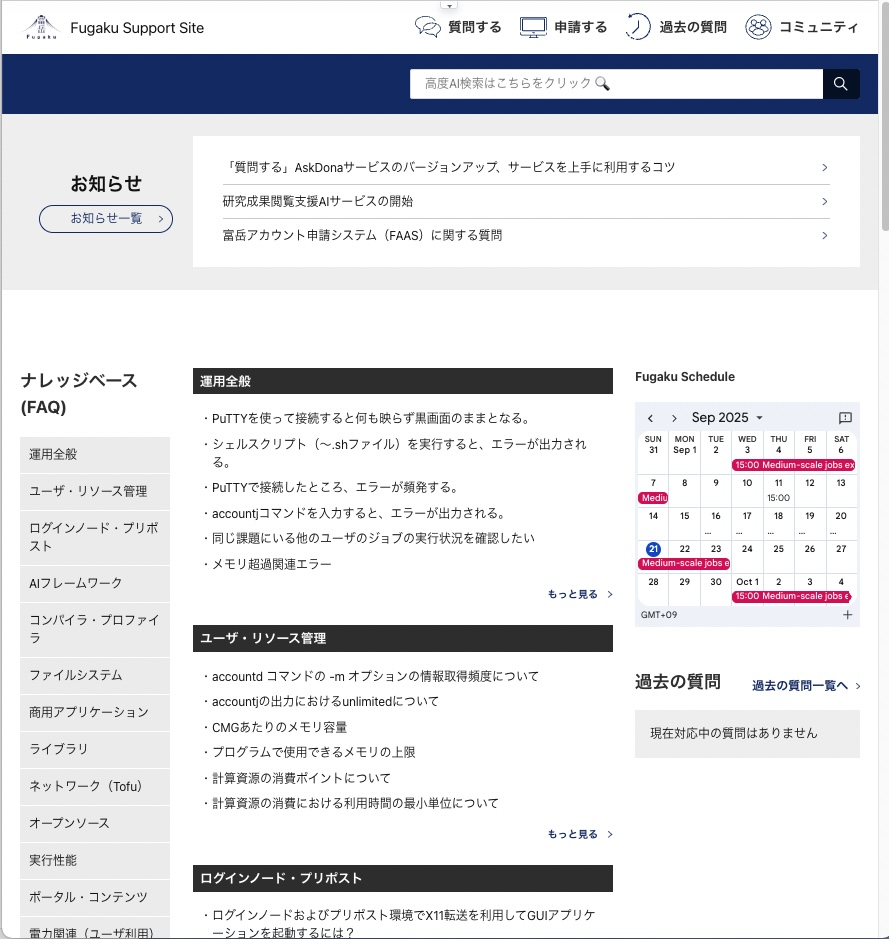
\includegraphics[width=\textwidth]{figs/FugakuSupportSite-Top.jpg}
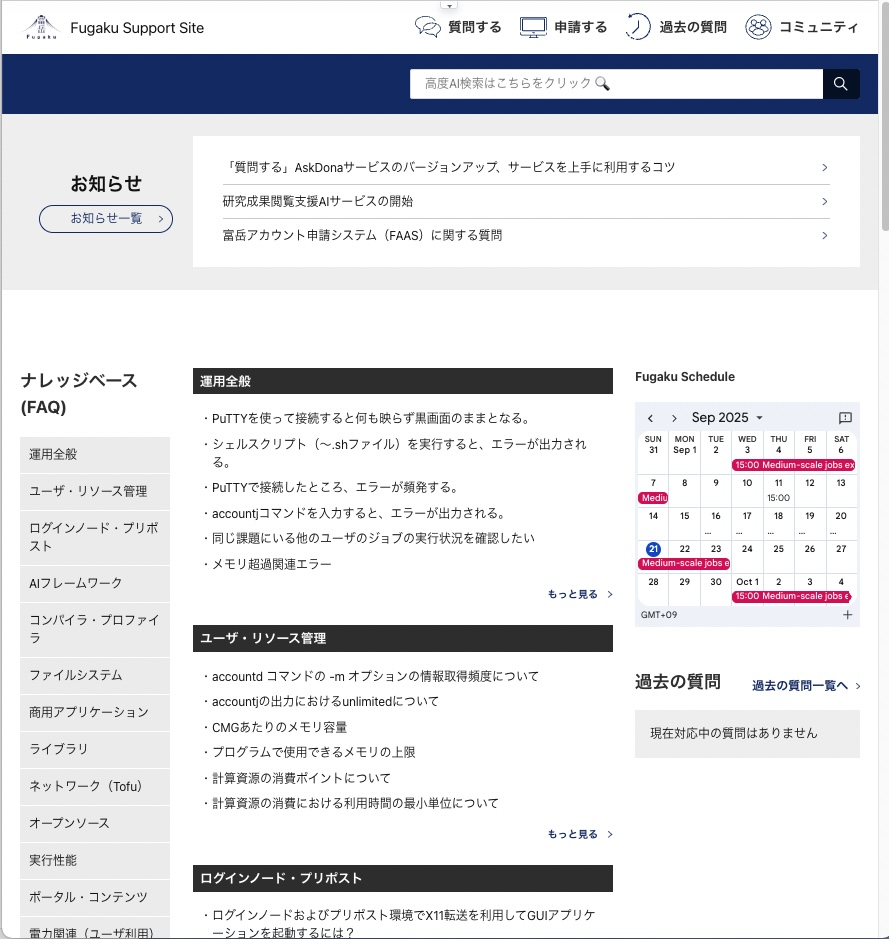
\includegraphics[width=8.5cm]{figs/FugakuSupportSite-Top.jpg}
\caption{富岳サポートサイトのUI}
\label{fig:FugakuSupport-SiteTop}
\end{figure}



\subsection{「富岳サポートサイト」への生成AI応用サービスの導入}

「富岳サポートサイト」でのFAQ記事を充実させてユーザへの情報提供を強化するという手法は妥当な手段であったと考えられるものの、FAQ記事数が300を超える様になると、多数の記事の中から自分にとって有用な情報にたどり着くことが容易とは言えない状況となってきた。
各FAQ記事をカテゴリごとに分類して検索が容易となる様なレイアウトを採用したり、記事の件名から本文内容を想起し易いように記述するなど、運用側での努力継続されているが、有用なFAQ記事により直接的にたどり着くための手法の検討が必要となった。

さらに根本的な課題として、ユーザが「富岳」を利用して目的とする計算ジョブを実行して成果を得るために、「富岳」の利用手引書・各種マニュアル・講習会資料・性能データ等の100冊以上の膨大なドキュメント類から自分が必要とする情報を探し当てて確認する作業が相当の負担となることであった。
この状況においては従来型のキーワード検索手法はユーザが意図する情報検索の手段としては不十分であることも指摘される。
例えば、ある技術的な事項が複数のマニュアルに記載されることもしばしばあるが、
それらの内容は同一の場合もあれば、用途に応じて焦点の当て方を変えた異なる説明方法となっていることもある。
さらには、調査したい事項そのものが概念として表現はできるが、具体的なキーワードとして想起できないという状況もしばしばある。

膨大な情報蓄積資源の中から、ユーザ自身にとって必要な情報を適切に得るための手段を提供すること、ひいてはユーザ自身による問題解決を促進することは「富岳」を運用するチームにとって重要な課題であった。

このような背景のもと、近年非常に進化が進んだ生成AIを応用した質問への自動回答および高度検索サービスの検討を2023年度から開始し、複数の生成AIサービス事業者による概念検証の実施、入札による事業者の決定を経て、2024年度に「富岳サポートサイト」へ「AIチャット」機能および「高度AI検索」機能としてサービスの追加を行なった。このプロセスの詳細は割愛するが、最終的に決定した事業者が著しいペースで進むAI技術分野の進化に伴い発生する様々な機能強化・改善要望に機動的に対応協力したことは、本サービスが定着する上での重要なポイントであった。



\section{生成AI AskDona}

「富岳サポートサイト」トップメニュー上段の「質問する」をクリックすると生成AI AskDonaのチャットセッションが開始される。
AskDonaのユーザインタフェイスを図\ref{fig:AskDona-Chat-1}に示す。


\begin{figure}[htbp]
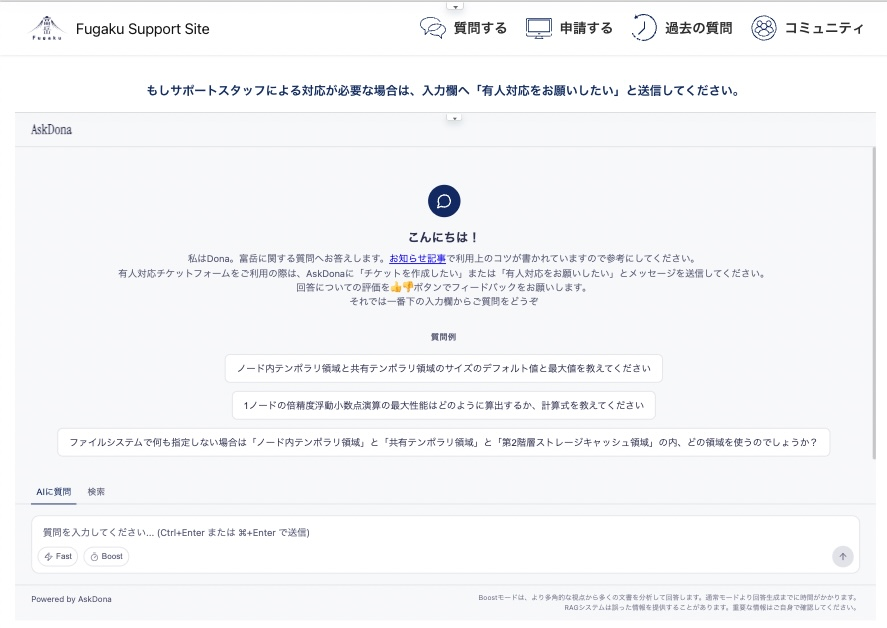
\includegraphics[width=8.5cm]{figs/AskDona-Chat-1.jpg}
\caption{生成AI応用サービスAskDonaのUI}
\label{fig:AskDona-Chat-1.jpg}
\end{figure}


\begin{figure}[htbp]
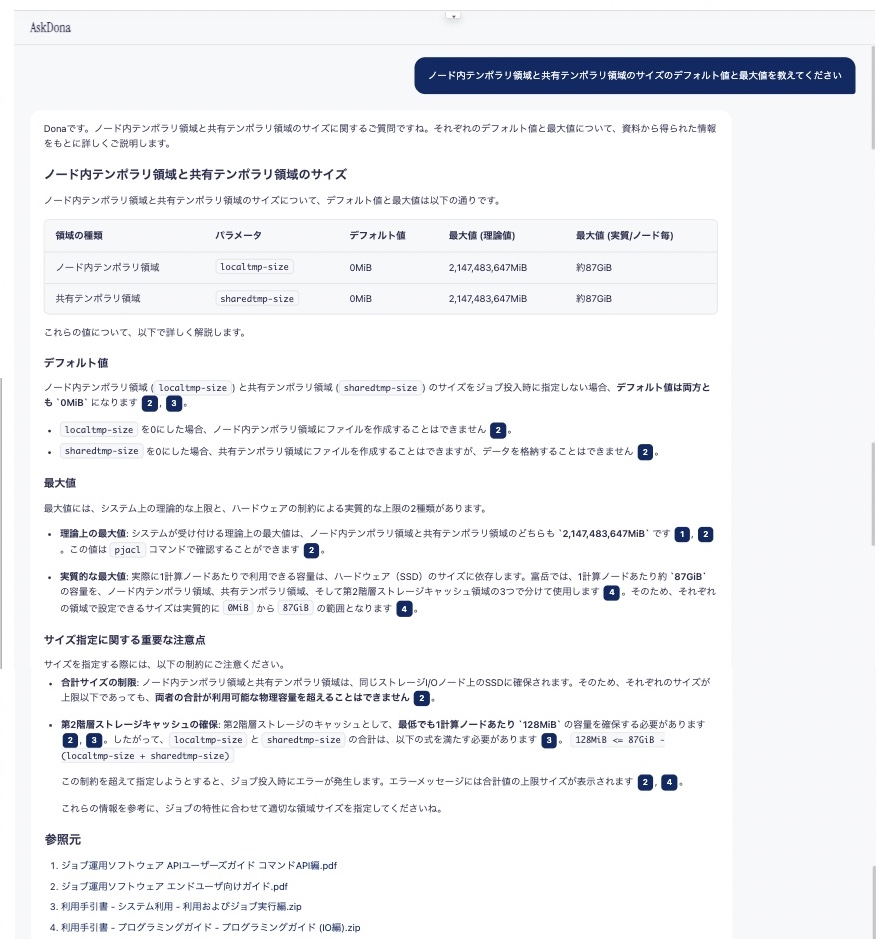
\includegraphics[width=8.5cm]{figs/AskDona-Answer.jpg}
\caption{AskDonaへの質問と解答例}
\label{fig:AskDona-Answer.jpg}
\end{figure}


論点:AskDonaの構成概要\\
論点:RAGのメリット(回答正解率の高さ、ハルシネーションが起きにくい構成)\\
論点:富岳サポートサイト専用の知識データベースの構築\\
論点:チケットサービスと生成AIチャット機能の統合\\
論点:個人情報の不所持方針\\


\section{生成AI導入の効果}

論点:発行チケット数の変化\\
論点:ユーザからのフィードバック\\
論点:ユーザの利用方法の変化\\
論点:課題:ユーザフィードバック率の低さ\\
論点:課題:人手で対応するチケットサービスの満足度V.S.生成AIサービスの満足度\\


\section{HPCI利用報告書の閲覧支援AIサービス}
論点:同じAI技術の水平展開\\
論点:HPCI利用課題の検索、論点整理、調査・比較\\
論点:JHPCN成果報告書の閲覧機能を追加\\


%参考文献
\begin{thebibliography}{99}
	\bibitem{refjournal} 雑誌の場合:著者名、タイトル、雑誌名 巻、号、ページ、発行年.
	\bibitem{refbook} 書籍の場合:著者名、書名、参照ページ、発行所、発行年.
\end{thebibliography}
\end{document}

% for vim cofiguration
% vim: set fileformat=unix fileencoding=utf8 filetype=tex
